
\section{Création de \\ Personnage}
\lettrine{L}{e} c\oe{}ur des jeux de rôle réside dans la possibilité de créer, améliorer et faire évoluer son propre personnage. Voilà comment ça fonctionne dans {\jedifont \doctitle}. 

\subsection{Les Attributs}
Chaque personnage commence le jeu avec d4 dans chaque Attribut et dispose de 5pt pour les améliorer. Améliorer l'un d'entre eux d’un type de dé (par exemple, de d4 à d6) coûte 1 point avec une limite : vous ne pouvez aller au-delà du d12.

\subsection{Compétences}
Les Compétences représentent les aptitudes apprises comme le Tir, le Combat, les connaissances professionnelles ou scientifiques et ainsi de suite. Elles sont générales et englobent tous les aspects qui leur sont reliés. Par exemple Tir englobe les fusils, les arcs, les lance-roquettes et toutes les armes à distance. Vous disposez de 15 points à répartir entre vos Compétences. Chaque dé de Compétence coûte 1 point (en commençant à d4) tant qu’il est inférieur ou égal à l’Attribut dont il dépend (noté entre parenthèses près du nom de la Compétence). Chaque dé de Compétence supérieur à l’Attribut dont il dépend coûte 2 points. De même que pour les Attributs, aucune Compétence ne peut dépasser d12.

\subsection{Atouts & Handicaps}
Faire naître un héro digne de ce nom ne se limite pas à lui faire grimper ses attributs et ses compétences. Ce qui fait la singularité d'un héro et qui le rend fun à jouer c'est ses Atouts et ses Handicaps. De la blonde très séduisante au Jedi Agè, vous prendrez toujours plus de plaisir à jouer un personnage unique dans ses détails que le jeune humain sans problème que vous êtes tout les jours.

Vous pouvez choisir jusqu’à 1 Handicap Majeur et 2 Handicaps Mineurs. Un Handicap Majeur donne 2 points et un Handicap Mineur 1 point.

Pour 2 points vous pouvez :
\begin{itemize}
    \item Augmenter un Attribut d’un type de dé (vous pouvez le faire avant de prendre vos Compétences).
    \item Choisir un Atout.
\end{itemize}

Pour 1 point vous pouvez :
\begin{itemize}
    \item Gagner un point de Compétence.
    \item Doubler vos fonds de départ (si vous débutez avec 500\$ vous obtenez 500\$ de plus).
\end{itemize}

\subsection{Races Jouables}
% To be balanced correctly, all races most have CAP +2
Vous pouvez choisir pour votre personnage n’importe quelle race disponible dans l'univers de Star Wars. L'orientation de chaque race est donnée à titre indicatif, chaque race possède des exceptions parmis ses héros.

\subsubsection{Humain}
\begin{samepage}
	\begin{flushright}
		\begin{tabular}{ l l }
			\textbf{Type} 			& Humanoïde \\
		   	\textbf{Planète} 		& Terre \\
		   	\textbf{Langage} 		& Basic \\
		   	\textbf{Orientation} 	& Neutre \\
		\end{tabular}
	\end{flushright}

	\vspace{-6\baselineskip}
	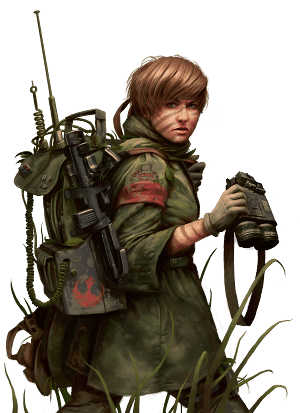
\includegraphics[width=5cm]{img/personnages/races/humain.png} 
\end{samepage}

Cette race comprend aussi bien les humains au sens strict (qu’ils soient originaires de Coruscant, de Correlia, de Kuat, de Naboo\ldots) que les humanoïdes dont les caractéristiques physiques, intellectuelles, sociales et culturelles sont suffisamment proches de celles des humains pour qu’il soit possible de les assimiler en termes de jeu.

\begin{description}[align=left]
\item [Adaptabilité] 	%CAP +2
	Les humains sont une race pleine de ressources, ils s’adaptent rapidement à toutes sorte de difficultés ou environnements.\\
	\emph{Compétence à d6}
\end{description}
\subsubsection{Barabel}
\begin{samepage}
	\begin{flushright}
		\begin{tabular}{ l l }
			\textbf{Type} 			& Reptile \\
		   	\textbf{Planète} 		& Barab I \\
		   	\textbf{Langage} 		& Barabel \\
		   	\textbf{Orientation} 	& Obscur \\
		\end{tabular}
	\end{flushright}

	\vspace{-5\baselineskip}
	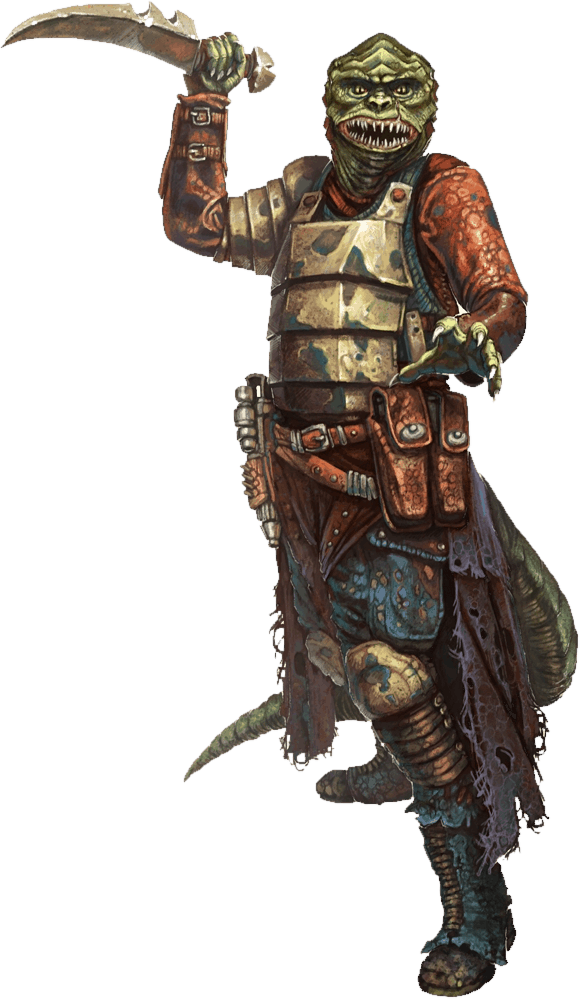
\includegraphics[width=5cm]{img/personnages/races/barabel.png}
\end{samepage}

Originaire de Barab I, les Barabels sont resté une race relativement primitive et isolée. Les Barabels vivent en clans dans un société principalement matriarcale. Ils sont fasciné par la guerre, la violence et les armes. Les Barabels ne sont pas profondément cruels mais il restent agressif de nature. En raison des nombreux rituels précédent les négociations, la diplomatie avec les Barabels est un exercice compliqué.

Le Barabel adulte est un reptile bipède dont la taille dépasse toujours les deux mètres. Sa dentition est formée d’une multitude de dents en forme d’aiguilles qui peuvent atteindre jusqu’à cinq centimètres de long et ses mains sont équipées de griffes puissantes.

\begin{description}[align=left]
\item [Enfance difficile] 	% CAP +1 +1
		De par l’environnement hostile de leur planète natale, les Barabels possèdent une résistance accrue à la chaleur et aux radiations.\\
		\emph{+4 en Résistance à la chaleur}\\
		\emph{+4 en Résistance aux radiations}
\item [\OE{il} Ophidien] 	% CAP +1
		Les yeux ophidiens du Barabel lui permettent de capter la plupart des ondes lumineuses allant du jaune à l’infrarouge mais il confond facilement les couleurs tirant dans les bleus et violets.\\
		\emph{Infravision}
\item [Arme naturelle]		% CAP +1
		Les mains des Barabels sont équipé de puissante griffes.\\
		\emph{For + d6 de dégâts}
\item [Balayage]			% CAP +2
		Les Barabels utilise leur appendice caudal d’instinct dans les combats.\\
		\emph{+ Atout Balayage}
\item [Primitif]			% CAP -3
		Les Barabels sont une race encore primitive.\\
		\emph{Int <= d6}
\item [Dur d’oreille]		% CAP -1
		Les Barabels en tant que reptilien ne possède pas d’oreille, il entendent par vibrations.\\
		\emph{Dur d’oreille (Mineur)}
\end{description}
\subsubsection{Bothan}

\begin{samepage}
	\begin{flushright}
		\begin{tabular}{ l l }
			\textbf{Type} 			& Félin \\
		   	\textbf{Planète} 		& Bothawui \\
		   	\textbf{Language} 		& Bothese \\
		   	\textbf{Orientation} 	& Lumineux \\
		\end{tabular}
	\end{flushright}

	\vspace{-5\baselineskip}
	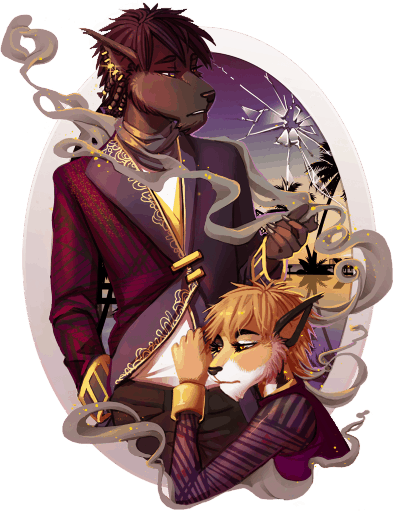
\includegraphics[width=5cm]{img/personnages/races/bothan.png}
\end{samepage}

Les Bothans sont des humanoïdes trappus, dont le corps est recouvert d'une épaisse fourrure pouvant varier du blanc-cassé à brun très foncé.
Le peuple bothan est originaire de la planète Bothawui, un monde cosmopolite épargné des troubles de la Guerre Civile Galactique en raison de la neutralité officielle du gouvernement bothan. Plusieurs colonies ont également été construites sur des planètes proches, telles que Kothlis, qui est désormais le siège d'une importante communauté. Toutes ces colonies forment l'Espace Bothan.\\
La structure sociale des Bothans est constituée par des clans familiaux, dont le nom est inclus dans le nom de chaque Bothan, à la suite d'une apostrophe.

\begin{description}[align=left]
\item [Agilité du Félin] 			% CAP +2
		Les Bothans possède la grace de leur ancêtres félins.\\
		\emph{Commence avec d6 Agi}
\item [Service de renseignement] 	% CAP +1
		Depuis plus de 300 ans ces êtres intelligents et rusés ont perfectionné leurs façons de faire, et ont développé un vaste réseau d'espions et d'informateurs destiné à recueillir toutes sortes d'informations sur les sujets les plus importants.\\
		\emph{d6 en Réseaux}
\item [Comme en plein jour] 		% CAP +1
		Grace à leur yeux de félins, les Bothans voient parfaitemnet dans l'obscurité.\\
		\emph{Vision Nocture}
\item [Déplacement rapide] 			% CAP +2
		Les Bothans, s'ils se baissent sur leur quatres pattes peuvent atteindre des vitesses de 80km/h.\\
		\emph{All = 10}
\item [Frêle] 						% CAP -2
		De contitution moins résistante, les Bothans sont moins adapté aux combats rapproché.\\
		\emph{-1 Résistance}
\item [Mauvaise réputation] 		% CAP -1
		Les ruses conduites par ce peuple, ainsi que l'opacité inhérente au Réseau Bothan, ne jouent pas en leur faveur. Certains leur reprochent de ne pas avoir prévu que l'Empire tendait une embuscade aux forces de l'Alliance.\\
		\emph{\'Etranger}
\item [Prudent] 					% CAP -1
		Les Bothans ne font rien à la légère, ils ne laissent nulle place au hazard et chaque décision est murrement réfléchie. Ils ne connaissent pas l'urgence.\\
		\emph{Prudent}
\end{description}
\subsubsection{Chiss}
\begin{samepage}
	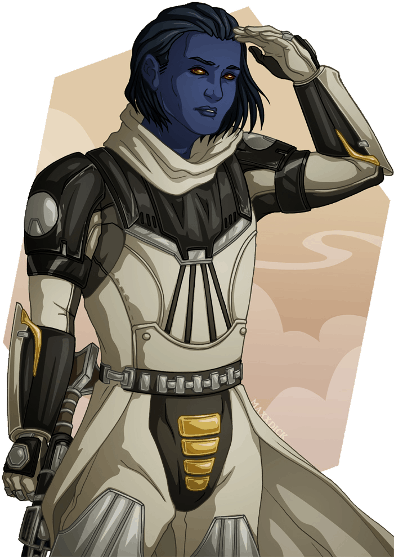
\includegraphics[width=5cm]{img/personnages/races/chiss.png}

	\vspace{-9\baselineskip}

	\begin{flushright}
		\begin{tabular}{ l l }
			\textbf{Type} 			& Humanoïde \\
		   	\textbf{Planète} 		& Csilla \\
		   	\textbf{Language} 		& Cheunh \\
		   	\textbf{Orientation} 	& Obscur \\
		\end{tabular}
	\end{flushright}
	\vspace{4\baselineskip}
\end{samepage}

Les Chiss font en moyenne 1,80m et ont une morphologie humaine. Cependant, il est impossible de les confondre à cause de leur peau bleue et de leurs yeux d’un rouge éclatant. Ils ont toujours des cheveux noirs, bien qu’avec les années, certains voient des cheveux blancs apparaitre. \\ 

La société Chiss est très évoluée. Ils ont de l’intérêt pour les arts et la science et maintiennent une puissante force militaire. Ils ont la réputation d’être de fins stratèges militaires mais leur façon de penser se retrouve dans tous les domaines de la vie quotidienne. Ils réfléchissent et pensent à différents points de vue et aux alternatives lorsqu’ils doivent prendre une décision.  

\begin{description}[align=left]
\item [Charismatique] 			% CAP +2 +2 +1
		Les Chiss sont des êtres charismatique habitué à commander des armées.\\
		\emph{+2 Cha}\\
		\emph{Commandement}\\
		\emph{d6 Connaissance (Combats)}
\item [Aquité visuelle] 		% CAP +1
		Les modifications qu’ont subies leurs yeux leur ont également donné une plus grande acuité visuelle.\\
		\emph{d6 Perception}
\item [Arrogant] 				% CAP -2
		Les Chiss sont fréquemment perçus par le reste de la galaxie, comme un peuple arrogant, calculateur et distant.\\
		\emph{Arrogant}
\item [Insensible à la Force] 		% CAP -1
		Les Chiss ne sont pas connus pour être une espèce sensible à la Force. Ils n’ont eut qu’un seul exemple d’individu sensible, en la personne de Sev’rance Tann. Cette dernière avait optée pour le côté obscur.\\
		\emph{A la création, l'augmentation de l'\^Ame coute 2pt}
\end{description}
\subsubsection{Droïde}
\begin{samepage}
	\vspace{4\baselineskip}
	\begin{tabular}{ l l }
		\textbf{Type} 			& Artificiel \\
	   	\textbf{Planète} 		& Multiple \\
	   	\textbf{Language} 		& Binaire \\
	   	\textbf{Orientation} 	& Neutre \\
	\end{tabular}

	\vspace{-11\baselineskip}

	\begin{flushright}
		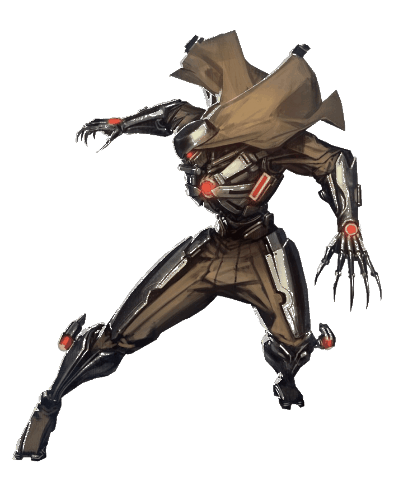
\includegraphics[width=6cm]{img/personnages/races/droide.png}
	\end{flushright}
	\vspace{-2\baselineskip}
\end{samepage}

Les Droïdes ne sont pas une race à proprement parlé mais des entités artificielles créés par d'autres races. Il peuvent être de Combat, de Protocole, de Compagnie, \ldots 
De par leur nature artificielle les Droïdes ne peuvent et ne pourront jamais utiliser la Force, c'est une notion qui leur est totalement étrangère.

\begin{description}[align=left]
\item [Créature artificielle] 	% CAP +2
		Les droides ne ressentent pas la douleur de blessures ou de la perte d'un membre.\\
		\emph{+2 pour se remettre d'un état secoué}\\
		\emph{Pas de bonus aux attaques ciblées}\\
		\emph{Pas de malus de blessure}
\item [Immunisé] 				% CAP +1
		Les maladies et les poisons sont sans effet sur les droides.\\
		\emph{Immunisé}
\item [Ambidextre] 				% CAP +2
		Un droïde ne fait pas de différence entre un membre et un autre, il peut utiliser n'importe lequel indistinctement.\\
		\emph{Ambidextre}
\item [Manque pas d'air] 		% CAP +2
		Les droïdes n'ont pas besoin de respirer, il peuvent stationné dans des lieux dépourvu d'atmosphère. Ils restent cependant sensible à la température.\\
		\emph{Ambidextre}
\item [Pas d'\^Ame] 			% CAP -3
		Il est impossible pour un droïde d'utiliser la force.\\
		\emph{\^Ame <= d6}
		\emph{Compétence Force interdite}
\item [Outsider] 				% CAP -2
		Le droïdes sont considéré comme des servants par les autres espèces, ils n'ont pas de droits et ne sont pas considéré comme faisant parti de la société.\\
		\emph{\'Etrangé}
\end{description}
\subsubsection{Gungan}
\begin{samepage}
	\vspace{-1\baselineskip}
	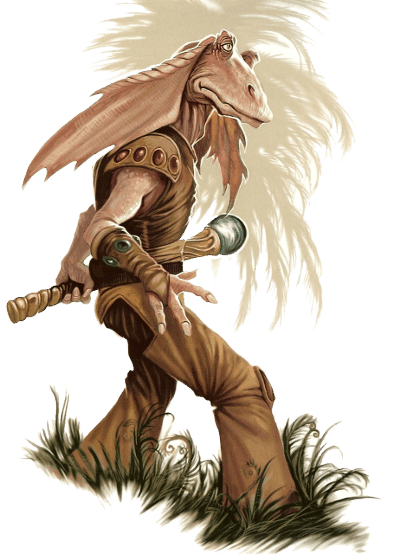
\includegraphics[width=6cm]{img/personnages/races/gungan.png}
	\vspace{-12\baselineskip}

	\begin{flushright}
		\begin{tabular}{ l l }
			\textbf{Type} 			& Amphibien \\
		   	\textbf{Planète} 		& Naboo \\
		   	\textbf{Language} 		& Gunganese \\
		   	\textbf{Orientation} 	& Lumineux \\
		\end{tabular}
	\end{flushright}

	\vspace{7\baselineskip}
\end{samepage}

Natifs de la planète Naboo, les Gungans vivent dans des cités sous-marines, évitant autant qu’ils le peuvent la race peuplant la surface : les Humains de Naboo. 

La physiologie d’un Gungan est de type humanoïde, quoique plus grand et plus fin qu’un Humain. Les Gungans possèdent de longues oreilles tombantes, des narines souples et des membranes rétractiles protégeant les yeux lors de leur déplacement aquatique. Leurs articulations sont libres et les ligaments très souples, permettant aux amphibiens de nager avec aisance sous l’eau.

La culture Gungan est une relation poussée entre la nature et l’individu. Ils essaient de ne pas utiliser la technologie.

\begin{description}[align=left]
\item [Aquatique] 			% CAP +2 +1
		Les gungans vivent dans les grandes étendues d’eau de Naboo, ils ne peuvent se noyer. Ils se déplace sous l’eau beacoup plus vite que n’importe qu’elle autre espèce.\\
		\emph{d6 Natation}\\
		\emph{Allure sous l’eau = d Natation}
		
\item [Mollusque] 			% CAP +3
		Leurs articulations sont libres et les ligaments très souples, permettant aux amphibiens de nager avec aisance sous l’eau. Cette souplesse leur permet de se faufiler dans des endroits étroits et d’esquiver les attaques avec plus de réussite.\\
		\emph{Esquive}
\end{description}
\subsubsection{Miraluka}
\begin{samepage}
	\vspace{-2\baselineskip}
	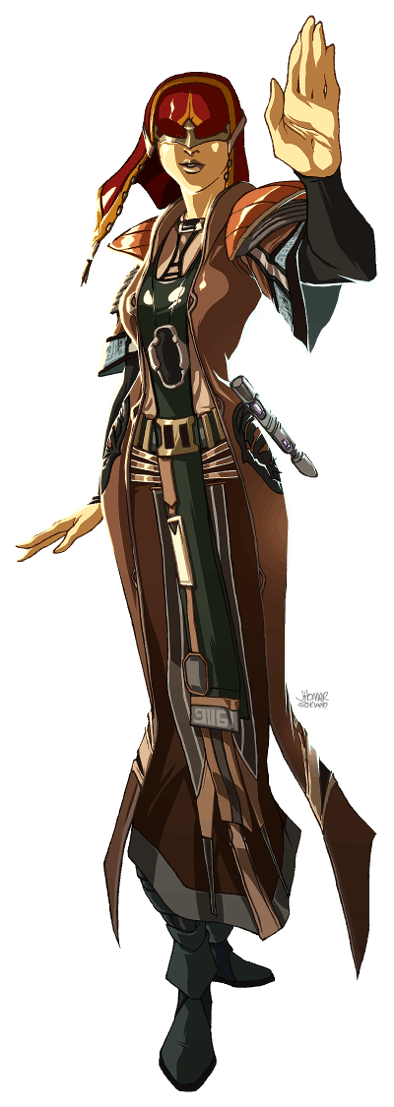
\includegraphics[width=4.5cm]{img/personnages/races/miraluka.png}

	\vspace{-5\baselineskip}

	\begin{flushright}
		\begin{tabular}{ l l }
			\textbf{Type} 			& Humanoïde \\
		   	\textbf{Planète} 		& Alpheridies \\
		   	\textbf{Langage} 		& Miralukese \\
		   	\textbf{Orientation} 	& Lumineux \\
		\end{tabular}
	\end{flushright}
\end{samepage}

Les Miraluka ressemblent beaucoup aux Humains mis à part le fait que leurs cavités oculaires sont vides et qu’ils sont capables de voir à travers la Force. A l’origine, les pacifiques Miraluka vivaient sur un monde dont le nom n’est pas passé à la postérité et qui entra dans une phase d’instabilité géophysique et géo-chimique durant laquelle l’atmosphère de la planète commença à s’évacuer dans l’espace. Des éclaireurs miraluka partirent à la recherche d’un monde où pourrait s’installer leur peuple et trouvèrent une planète habitable dans le système d’Abron : Alpheridies. 

Les Miraluka ont également tendance à masquer le haut de leur visage avec des viseurs ou des morceaux de tissus pour dissimuler leurs orbites vides, en particulier lorsqu’ils voyagent, pour ne pas attirer l’attention.


\begin{description}[align=left]
\item [Sensibilité raciale à la force] 	% CAP +2
		Il est extrêmement rare qu’une espèce toute entière soit sensible aux flux de la Force et il n’est guère étonnant que certains Miraluka, parmi ceux qui maîtrisaient le mieux la Force, aient rejoint l’Ordre Jedi.\\
		\emph{d6 \^Ame}

\item [Vision de force] 			% CAP +2 +2
		Ils perçoivent leur environnement grâce à la Force. Cette « vision » est si puissante que s’ils « regardent » un Jedi ou un Sith à travers elle, ils verront les radiations de Force qu’ils dégagent. Il faut néanmoins noter que la connexion à la Force varie en fonction de chaque Miraluka.\\
		\emph{d6 compétence Force}\\
		\emph{Pouvoir (Vision de Force) permanent et gratuit}

\item [Aveugle dans la lumière] 	% CAP -2 -2
		Du fait qu’ils n’aient pas de globe oculaire, les Miraluka voient par la force, tout ce qui n’est pas lié à la Force leur échappe. Les droïdes, par exemple, étant des "vides de Force" ne leur apparaissent pas. Il leur est impossible de lire.\\
		\emph{Handicap (Aveugle)}\\
		\emph{-1 Parade}
\end{description}
\subsubsection{Togruta}
\begin{samepage}
	\begin{tabular}{ l l }
		\textbf{Type} 			& Humanoïde \\
	   	\textbf{Planète} 		& Shili \\
	   	\textbf{Language} 		& Togru \\
	   	\textbf{Orientation} 	& Lumineux \\
	\end{tabular}

	\vspace{-9\baselineskip}
	\begin{flushright}
		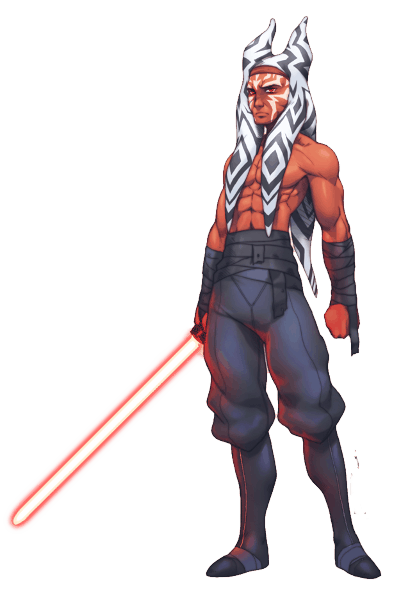
\includegraphics[width=7cm]{img/personnages/races/togruta.png}
	\end{flushright}

	\vspace{-2\baselineskip}
\end{samepage}

Les Togrutas sont des humanoïdes dont l'apparence induit souvent en erreur les observateurs peu attentifs et les fait passer pour des Twi'leks. Ils possèdent une couleur de peau rouge vif, de la même manière là encore que certaines sous-espèces de Twi-leks. Leurs yeux sont entourés d'un grand cercle blanc, et leurs montrals sont également de cette couleur. Enfin leurs lekkus sont bariolés, de manière à assurer un camouflage efficace. Le Togruta adulte atteint en général une taille moyenne de 180 cm. 


\begin{description}[align=left]
\item [Agilité] 				% CAP +2
		Les Togrutas sont des être particulièrement agile.\\
		\emph{d6 \^Agi}
\item [Montrals] 				% CAP +1 +2
		Les montrals des Togrutas renferment de puissants organes sensoriels qui réagissent aux ultrasons. En pratique cela leur permet de se repérer dans leur environnement de manière efficace et autonome, ainsi que de détecter la présence d'éventuels prédateurs sur leur monde natal, Shili..\\
		\emph{d6 Perception}\\
		\emph{Sixieme Sens}
\item [Predateur né] 			% CAP +1
		Les Togrutas sur leur planète d'origine sont des prédateurs habitué à chasser. Ils aiment leur proies fraiche.\\
		\emph{d6 Discrétion}
\item [Mauvaise réputation] 	% CAP -1
		Leur réputation n'est pas toujours excellente car des rumeurs anciennes prétendent que les Togrutas sont capables d'injecter un poison mortel à leur victime, ce qui incite évidemment à la méfiance.\\
		\emph{\'Etranger}
\item [Frèle] 					% CAP -2
		Les Togrutas sont de corpulence élancé et sont moins résistant que d'autres races.\\
		\emph{-1 Résistance}
\item [Un pour tous] 			% CAP -1
		Les Togrutas sont une espèce très loyale envers leur compagnons d'aventure, en laisser un dans l'embarras alors qu'il y avait une chance même minime de le sauver est impensable.\\
		\emph{Loyal}
\end{description}
\subsubsection{Twi'Lek}
\begin{samepage}
	\vspace{-1\baselineskip}
	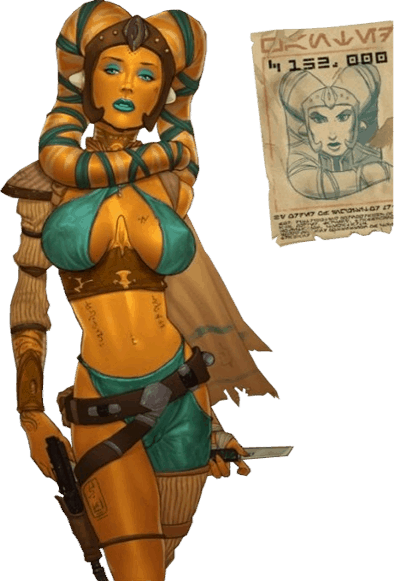
\includegraphics[width=6cm]{img/personnages/races/twilek.png}
	\vspace{-5\baselineskip}
	\begin{flushright}
		\begin{tabular}{ l l }
			\textbf{Type} 			& Humanoïde \\
		   	\textbf{Planète} 		& Ryloth \\
		   	\textbf{Language} 		& Ryl \\
		   	\textbf{Orientation} 	& Neutre \\
		\end{tabular}
	\end{flushright}
\end{samepage}

Les Twi'leks sont de grands humanoïdes, dont la peau très pigmentée peut avoir différentes couleurs selon les individus : rouge, jaune ou encore bleue par exemple. Leur trait le plus caractéristique est la paire de tentacules, appelés "lekkus", qui prend sa base au sommet de leur crâne.

Les Twi'leks utilisent leurs lekkus quand ils parlent leur langage d'origine, le twi'leki. Il s'agit d'un langage combinant communication orale et gestes, les mots étant accompagnés et complétés par les mouvements des lekkus.

La société twi'lek est divisée en deux castes très distinctes : les marchands et les guerriers.

% Les Twi'leks sont une race spéciale puisque c'est la seule à proposer des capacités différente pour les mâles et pour les femelles de la race. Attention toutefois à ce que les deux restent équilibré et à ne pas dépasser les +2 de capacité sans quoi les mâles et les femelles seraient trop différents.
\begin{description}[align=left]
\item [Rusé \& Astucieux] 			% CAP +2
		Les Twi'leks n'ont jamais eu la vie facile, entre leur monde natal pas vraiment amical et les hordes de criminels qui en veulent à leur Ryll, il leur a fallu faire preuve d'astuce pour composer avec tout cela.\\
		\emph{d6 Int}
\item [Ni chaud ni froid] 			% CAP +2
		Ryloth la terre natale des Twi'leks est composé de deux faces, l'une en permanence au soleil, à près de 300° et l'autre en permance dans l'obscurité. Le tout parcouru par de violentes tempêtes. Des conditions qui font des natifs des êtres particulièrement résistants à leur environnement.\\
		\emph{+4 pour résister aux effets négatifs de l’environnement}
\item [Lekkus Speaking] 			% Gratuit
		En plus du Ryl, les Twi'leks, grâce à leur lekkus sont capable de parler le twi'leki, ce qui s'avère difficile pour les autres races.\\
		\emph{Connaissance (twi'leki)}
\item [Belle plante (Femelles)] 	% CAP +2
		Toutes les femelles Twi'lek sont belle, au point que leur propre mâle les vendent aux pirates et autres criminels de passage pour arrondir les fins de mois.\\
		\emph{Séduisant (Cette capacité ne s'applique qu'aux personnages de sexe féminin)}
\item [Immunisé (Mâles)] 			% CAP +2
		Physiologiquement, les Twi'leks sont capables de résister à certaines toxines et maladies.\\
		\emph{Guérison rapide (Cette capacité ne s'applique qu'aux personnages de sexe masculin)}
\item [Frêles] 						% CAP -2
		Les Twi'leks sont de constitution moins résistance que les autres races.\\
		\emph{-1 Résistance}
\item [Prudent] 					% CAP -1
		Les Twi'leks en êtres intelligent prennent le temps de la réflexion et ne font pas les choses sans y réfléchir avant.\\
		\emph{Prudent}
\item [Hutt(er)] 					% CAP -1
		Les problèmes liés au commerce du Ryll ont obligé les Twi'lek à vendre leurs femmes pour présever leur monde des criminels. Les Hutt sont les premiers client de ce traffic et les Twi'leks libre ont du mal à garder leur calme face à un Hutt.\\
		\emph{Ennemi Racial (Hutt)}
\end{description}
\subsubsection{Wookie}
\begin{samepage}
	\begin{flushright}
		\begin{tabular}{ l l }
			\textbf{Type} 			& Bipèdes \\
		   	\textbf{Planète} 		& Kashyyyk \\
		   	\textbf{Language} 		& Shyriiwook \\
		   	\textbf{Orientation} 	& Lumineux \\
		\end{tabular}
	\end{flushright}
	\vspace{-6\baselineskip}
	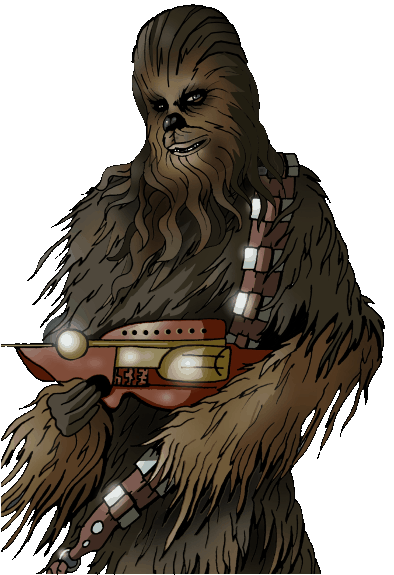
\includegraphics[width=6cm]{img/personnages/races/wookie.png}
\end{samepage}

Les Wookies sont de grand bipèdes à fourrure dépassant couramment les deux mètres de haut. Ils sont originaires de la planète Kashyyyk et n'ont que très peu de communautés en dehors de leur monde natal. Capables de vivre plusieurs siècles, les Wookies sont également dotés de longues griffes rétractiles, qu'ils utilisent principalement pour s'accrocher à la végétation dense de Kashyyyk. Leur honneur leur interdit cependant formellement d'utiliser ces griffes comme armes lors d'un combat.

\begin{description}[align=left]
\item [Force de la nature] 				% CAP +2
	L'imagerie populaire veut que les Wookies soit physiquement la race la plus forte de la galaxie (en tous cas, par rapport à sa taille).\\
	\emph{d6 For}
\item [Increvable] 						% CAP +2 +3
	Les Wookies possèdent, entres autres, de remarquables capacités de récupération, et sont capables de survivre à des blessures très graves.\\
	\emph{Increvable}\\
	\emph{Combatif}
\item [Shyriiwook] 						% CAP -1
		Les Wookies parlent entre eux leur langage, le Shyriiwook, un dialecte très complexe, en raison du mélange de feulements, rugissements, gestes et autres bruits nécessaires à son usage.\\
		\emph{Ne parle pas le Basic}
\item [Force \& Honneur] 				% CAP -2
	Comme de nombreux peuples mettant en avant des valeurs comme l'honneur, les Wookies pratiquent les serments et la "dette de vie". Celle-ci peut les amener à défendre jusqu'à la mort un étranger (même d'une autre race) auquel ils pensent devoir une grande faveur. Une dette de vie est définitive et rien ne peut la lever.\\
	\emph{Code d'honneur}
\item [Ennemis jurés] 					% CAP -1
	Les ennemis jurés des Wookies, les Trandoshans, se firent à cette époque un malin plaisir à chasser et à capturer les wookies.\\
	\emph{Ennemi Racial (Trandoshans) -4 Cha}
\item [Il faut partir à point] 			% CAP -1
	De par leur stature, les Wookies ne sont pas les êtres les plus vif de la galaxy.\\
	\emph{Allure 5}
\end{description}
\subsubsection{Zabrak}
\begin{samepage}
	\begin{flushright}
		\begin{tabular}{ l l }
			\textbf{Type} 			& Humanoïde \\
		   	\textbf{Planète} 		& Iridonia \\
		   	\textbf{Langage} 		& Zabraki \\
		   	\textbf{Orientation} 	& Obscur \\
		\end{tabular}
	\end{flushright}
	\vspace{-6\baselineskip}
	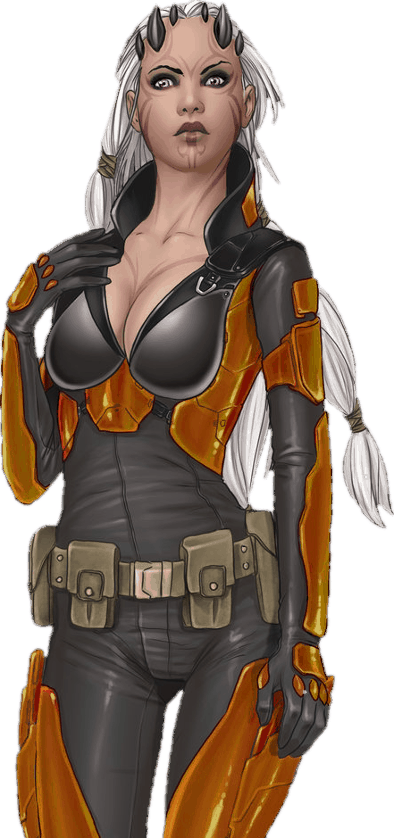
\includegraphics[width=5cm]{img/personnages/races/zabrak.png}
\end{samepage}

Originaires de la planète Iridonia, les Zabraks sont des humanoïdes d’une taille pouvant aller de 1,60 mètre à 2,10 mètres, et dont la tête était recouverte de petites cornes et le corps de tatouages, qui donnent à cette espèce un aspect parfois effrayant. Très tôt dans l’histoire galactique les Zabraks ont atteint un niveau de technologie élevé et ont pu coloniser plusieurs mondes extérieurs aux alentours de leur planète natale. On estime que cette espèce a ainsi établi huit colonies dans la Bordure Extérieure, et que les différents groupes coloniaux ont pu prospérer de façon suffisamment importante pour que les Zabraks s’identifient eux-même selon les colonies d’où ils viennent, plutôt que par rapport à Iridonia uniquement.

\begin{description}[align=left]
	\item [Endurance] 				% CAP +2
		Très tôt dans l’histoire galactique les Zabraks ont atteint un niveau de technologie élevé et ont pu coloniser plusieurs mondes extérieurs aux alentours de leur planète natale. Cette vague de colonisation à forcé l’espèce à s’adapter et à se renforcer.\\
		\emph{d6 Vig}

	\item [Braveheart] 				% CAP +2 +1
		Les Zabraks sont des explorateurs courageux et des guerriers que rien n’effraie.\\
		\emph{Atout (Brave)}\\
		\emph{d6 Combat}

	\item [Survivor] 				% CAP +1
		Les Zabraks présentent un instinct de survie supérieur à la plupart des autres espèces.\\
		\emph{d6 Survie}

	\item [Fierté mal placé] 				% CAP -2 -2
		Les Zabraks dans leur ensemble possèdent un fort caractère et une volonté de fer.\\
		\emph{Handicap (Présomptueux)}
		\emph{Handicap (Arrogant)}
\end{description}

%\subsection{Races Non Jouables}
%\input{chapitres/personnages/races/hutt}
%\input{chapitres/personnages/races/jawa}
\clearpage
\subsection{Compétences}
Vous trouverez ici les Compétences utilisables\footnotemark[1] dans \swfe. L’utilisation d’une Compétence en situation normale ne devrait pas donner lieu à un jet de dé. Seules les situations de stress, lorsque le temps est compté ou que la réussite est loin d’être acquise, devraient donner lieu à un test de Compétence.

\footnotetext[1]{Seules les compétences modifiés sont détaillés ici, pour les autres, elles sont décritent dans le bouquin de Savage Worlds.}

\begin{description}[align=left]
    \item [Combat (Agi)]
        Combat englobe toutes les attaques de corps à corps quelle que soit l’arme de mêlée utilisée.

    \item [Conduite (Agi)]
        Conduite permet à votre héros de conduire les véhicules terrestres ou aéroglisseurs courants de l'univers Star Wars.

    \item [Connaissance (Int)]
        Connaissance est une Compétence passe-partout qu’il faut spécialiser. Elle inclue aussi les langues autre que la langue natale et le Basic.

    \item [Piratage (Int)]
        L'utilisation d'un ordinateur, la manipulation de serrure électronique ou tout autre appareil informatique est couvert par cette compétence.

    \item [Discrétion (Agi)]
        Discrétion représente la faculté de se cacher et de se déplacer en silence, mais aussi de camoufler des objets ou de subtiliser de petits objets à l’insu de tous.

    \item [Équitation (Agi)]
        Équitation permet de monter, contrôler et chevaucher tout animal domestiqué.

    \item [Escalade (For)]
        Les personnages peuvent être amenés à escalader des obstacles ou grimper une falaise pour prendre l'avantage du terrain lors d'une attaque, ou encore pour échapper à un ennemi trop coriace.

    \item [Maîtrise de la Force (\^Ame)]
        C'est la compétence qui mesure le niveau de votre héro à l'utilisation de la Force. Cette compétence ne sert à rien sans l'Atout Arcane (Force).

    \item [Intimidation (\^Ame)]
        Intimidation est l’art d’effrayer un adversaire par la force de sa volonté, que ce soit par une menace ouverte ou voilée ou tout simplement avec un énorme flingue.

    \item [Jeu (Int)]
        Voici un moyen rapide pour simuler une demi-heure d’une partie de jeu sans lancer les dés pour la moindre phase du jeu en question.

    \item [Lancer (Agi)]
        Lancer s’applique à toutes les armes qui se lancent, grenades, couteaux, haches, lances, etc.

    \item [Natation (Agi)]
        Natation détermine si un personnage nage ou coule comme une pierre lorsqu’il se trouve dans l’eau, ainsi que sa vitesse de déplacement en milieu aquatique.

    \item [Navigation (Int)]
        Navigation est la capacité du personnage à voyager et a se repérer dans l'espace. Il englobe aussi l'entretien journalier de l'équipement utilisé.

    \item [Perception (Int)]
        Perception représente la vigilance d’un héros et son habilité à découvrir objets ou indices.

    \item [Pilotage (Agi)]
        Pilotage permet d’utiliser tous les types d’appareils aériens ou spatiaux communs.

    \item [Pistage (Int)]
        Pistage permet de suivre les traces d’un ou de plusieurs individus sur tout type de terrain.

    \item [Recherche (Int)]
        Recherche permet d’obtenir des informations avec une bibliothèque, HoloNet, les journeaux ou toute autre source écrite.

    \item [Réparation (Int)]
        Réparation représente la capacité à remettre en état gadgets, véhicules, armes et autres machines.

    \item [Réseaux (Int)]
        Réseaux permet d’obtenir des informations dans la rue, les bars ou par des contacts en utilisant la menace, la corruption ou en offrant des verres. Cette compétence peut aussi représenté les informateurs du héro.

    \item [Sarcasme (Int)]
        Sarcasme est une attaque contre l’amour-propre d’un individu en le ridiculisant par la parole ou le geste.

    \item [Soins (Int)]
        Soins consiste à savoir comment guérir les plaies et traiter les blessures.

    \item [Survie (Int)]
        Survie permet de trouver nourriture, eau ou abri en milieu hostile.

    \item [Tir (Agi)]
        Tir concerne toute tentative pour toucher une cible avec n’importe quelle arme à distance (arc, pistolet, lance-roquettes, etc\ldots).
\end{description}

\begin{paperbox}{Piratage}
    Cette compétence vient remplacer le Crochetage qui dans Star Wars n'a pas une grosse utilité. La compétence Piratage (Informatique) va s'utiliser de la même façon mais sur l'Inellect au lieu de de l'Agilité. L'informatique pourra être utilisé dés qu'un ordinateur entre en scène. On pourra par exemple déverrouiller des sas de vaisseau ou stoppé un signal d'alarme ou encore désactiver des capteurs à plus haut niveau.

    Les Droïde n'en sont pas systématiquement pourvu, cela dépend de leur programmation.
\end{paperbox}

\begin{paperbox}{Navigation}
    La navigation exite mais son domaine d'application change un peu, on ne parle pas dans Star Wars de bateau mais de vaisseaux spatiaux. La navigation est alors la capacité du héro à s'orienter dans le vide cidéral. Mais cela s'applique aussi au sol pour se repérer sur une carte par exemple.
\end{paperbox}

\clearpage
\subsection{Handicaps}

Les Handicaps\footnotemark[1] représentent les défauts qui compliquent parfois la vie de votre personnage. Certains sont plus contraignant que d'autres et certains dépendent du scénario. Ils permettent de choisir des Atouts supplémentaires mais surtout ajoute du caractère à votre personnage et augmente ainsi sont intérêt et votre plaisir de jouer.

\footnotetext[1]{Comme dit en préambule, le but de ce manuel est d'être suffisant pour qu'un joueur puisse créer sa ficher de personnage. Pour cela, les handicaps ont été recopié bètement, sauf pour les nouveaux biensûr.}

\begin{description}[align=left]
    \item [Âgé (Majeur)]
        Votre héros se fait vieux, certes, mais n'est pas encore prêt pour l'hospice. Son Allure est réduite de 1. Sa Force et sa Vigueur diminuent d’un type de dé (selon l'age, minimum d4). Elles ne pourront plus jamais être élevées. Le côté positif, c’est que l’expérience de l'âge lui rapporte 5 points de Compétences supplémentaires à répartir sur toutes Compétences liées à l'Intellect.

    \item [Anémique (Mineur)]
        Votre héros est particulièrement sensible aux maladies, à la fatigue et aux effets de l'environnement. Il subit un malus de -2 à tous les jets de Vigueur pour résister à la fatigue, au poison, aux maladies, etc\ldots

    \item [Arrogant (Majeur)]
        Votre héros ne pense pas qu'il est le meilleur, il le sait. Quel que soit le domaine nul ne peut le battre et il le prouve à chaque occasion. Gagner ne lui suffit pas. Il doit totalement dominer son adversaire. Si un adversaire doute de sa supériorité, il cherchera à l'humilier et à lui prouver qu'il peut le battre quand il veut.\\
        Les héros Arrogants cherchent toujours le chef adverse dans un combat, n'attaquant ses subalternes que s'ils se mettent en travers de leur chemin.

    \item [Aveugle (Majeur)]
        Votre héros est complètement aveugle. Il subit un malus de -6 à toutes les tâches nécessitant la vue (à peu près toutes ou presque) et -2 à toutes les interactions en société (il ne peut pas déchiffrer les expressions de ses interlocuteurs). Le bon côté, c'est que les personnages Aveugles obtiennent un Atout supplémentaire de leur choix pour compenser cet Handicap particulièrement pénalisant.

    \item [Bavard (Mineur)]
        On dit qu'une grande gueule peut couler un navire. Votre héros l'est au point qu'il pourrait couler une armada. Il ne sait pas garder un secret, il dévoile tout les plans et même les secrets les mieux gardés de ses amis et choisit toujours le plus mauvais moment pour le faire.

    \item [Bizarrerie (Mineur)]
        Votre héros possède une bizarrerie, rien de grave, mais pouvant lui causer des ennuis. Un escrimeur qui tente d'abord de zébrer ses initiales sur ses ennemis avant de les attaquer, un nain se vantant sans cesse de sa culture ou une jeune snob qui refuse de s'assoir, boire ou manger avec les gens de classe inférieure sont tous des exemples bizarrerie.

    \item [Boiteux (Majeur)]
        Une vieille blessure a presque estropié votre héros. Son Allure est réduite de 2 et il n'utilise qu'un d4 pour courir. L'Allure d’un personnage ne peut jamais passer en dessous de 1.

    \item [Borgne (Majeur)]
        Votre héros a dans le passé eu l'\oe{il} crevé par un ennemi. S'il ne porte pas un bandeau ou un \oe{il} de verre (d'un prix de l'ordre de 500 Cr) il subit -1 à son Charisme à cause de sa vilaine blessure. Il subit -2 à tout jet de Trait nécessitant une perception de la profondeur (Tirer, Lancer, sauter d'un mât à l'autre et ainsi de suite).

    \item [Chimères (Mineur ou Majeur)]
        Votre héros croit en des choses qui paraissent étranges pour les autres. Les Chimères Mineures sont inoffensives ou alors le personnage y fait rarement allusion (les chiens parlent, on est tous des personnages d'un jeu bizarre, etc\ldots).\\
        Avec une Chimère Majeure, il exprime souvent ses opinions sur le sujet et cela peut s'avérer dangereux (je suis allergique aux armures, les Vong sont mes amis, \ldots).

    \item [Couard (Majeur)]
        Tout le monde n'a pas des nerfs d'acier. Votre héros blêmit à la vue du sang et est terrifié à l'idée même de subir une blessure. Tous ses tests de terreur subissent un malus de -2.

    \item [Code d'Honneur (Majeur)]
        L'honneur est très important aux yeux de votre personnage. Il n'a qu'une parole, traite ses prisonniers avec décence et se conforme d'ordinaire aux codes de bonne conduite et règles de bienséance de son monde.

    \item [Cupide (Mineur)]
        Votre héros est un grippe-sou qui mesure sa valeur en trésor.

    \item [Curieux (Majeur)]
        C'est un vilain défaut et votre personnage est très vilain. Les personnages Curieux sont facilement attirés par l'aventure. Il faut qu'ils fouillent partout et désirent toujours savoir ce qui se cache derrière chaque mystère.

    \item [Deux mains gauches (Mineur)]
        Certaines personnes ne sont tout simplement pas douées avec la technologie. Un personnage affligé de ce défaut subit systématiquement un malus de -2 à ses jets de Réparer. Et chaque fois qu'il utilise un appareil technologique, un résultat de 1 sur son dé de Compétence (sans tenir compte du dé Joker) signifie que l'appareil se détraque. Le remettre en état nécessitera un jet de Réparer à -2 et 1d6 heures de travail.

    \item [Dur d’Oreille (Mineur ou Majeur)]
        Un personnage ayant perdu tout ou partie de son acuité auditive possède ce handicap. Un Handicap Mineur fait subir -2 à tous ses jets de Perception liés à l'audition y compris se réveiller à cause du bruit. Un Handicap Majeur signifie que le personnage est sourd et rate automatiquement tous ses jets de Perception liés à l'audition.

    \item [Ennemi (Mineur ou Majeur)]
        Quelqu'un quelque part déteste votre héros et veut sa mort. Le niveau du Handicap dépend de la puissance de l'ennemi et de sa fréquence d'apparition. Un Ennemi Mineur sera un chasseur de prime solitaire avide de vengeance. Un Ennemi Majeur sera un seigneur Sith démoniaque vouant une haine implacable envers votre héros.\\
        Si l'Ennemi est vaincu le MJ s'arrange pour lui trouver un remplaçant à moins que le héros n'efface le Handicap en sacrifiant une Progression.

    \item [Étranger (Mineur)]
        Votre héros n'appartient pas à la société dans laquelle il vit. Un Wookie sur Ryloth, un Gungan au sénat, .... Les marchands augmentent leurs prix pour le personnage, lui refusent leur aide et le traitent comme s'il était d'un rang inférieur. \\
        En plus des effets de roleplay ci-dessus, le Charisme de votre héros subit tout le temps un malus de -2, sauf quand il est parmi ses semblables.

    \item [Frêle (Majeur)]
        Votre héros est, soit très petit, soit très maigre, voire les deux par rapport à la norme de son peuple. Sa Résistance est réduite de 1 à cause de sa faible stature.

    \item [Mal de l'espace (Mineur)]
        Votre héros ne supporte pas les voyages à vitesses super luminique. Quelque chose dans les déplacements en hyperespace le rend malade. Après chaque déplacement hyperespace, il souffre d'un niveau de fatigue pendant 24h. Les voyages en hyperespace peuvent l'affaiblir mais pas le tuer.

    \item [Gamin (Majeur)]
        Il arrive que des événements incroyables poussent des enfants vers l'aventure. Sachez que choisir ce Handicap signifie débuter avec un gros désavantage. Les héros Gamins ont entre 8 et 12 ans (en âge humain. Adaptez en fonction des races où les tranches d'âge sont différentes). Ils ne disposent que de 3 points à investir dans leurs Attributs et de 10 points dans leurs Compétences.\\
        Le bon côté de la chose, c'est que les Gamins ont beaucoup de chance. Ils débutent chaque session de jeu avec un Jeton en plus. Ce dernier est cumulable avec les autres Jetons attribués par les Atouts Chanceux ou Très Chanceux. Quand votre héros arrive à maturité, ce Handicap disparaît naturellement. Il en a déjà bien payé le prix. Il n'obtient plus non plus le Jeton offert par le Handicap lorsqu'il atteint l'âge de 18 ans (ou équivalent pour une autre race).

    \item [Héroïque (Majeur)]
        Votre héros ne dit jamais non à une personne dans le besoin. Cela peut ne pas lui plaire mais il se sent obligé de secourir ceux qu'il considère sans défense. C'est le premier à se jeter dans un immeuble en flammes, à accepter de chasser les monstres pour trois fois rien et ne pas savoir résister aux larmes d'une belle infortunée.

    \item [Ignorant (Majeur)]
        Votre héros en sait moins que les autres sur le monde dans lequel il vit. Il subit un malus de -2 aux jets de Culture générale.

    \item [Illettré (Mineur)]
        Votre héros ne sait pas lire. Il peut écrire son nom et sait ce qu'un panneau STOP signifie, mais c'est à peu près tout. Les maths ne sont pas son fort non plus. 2 + 2 = 4 passe encore mais ne lui parlez pas de multiplication. Les Illettrés ne savent ni lire, ni écrire, quel que soit par ailleurs le nombre de langues qu'ils savent parler.

    \item [Loyal (Mineur)]
        Votre personnage n'est peut-être pas l'archétype du héros, mais il donnerait sa vie pour ses amis. Il est incapable de laisser tomber ses compagnons s'il a la moindre possibilité de leur venir en aide.

    \item [Malchanceux (Majeur)]
        Votre héros est moins chanceux que les autres. Il reçoit un Jeton de moins par session de jeu. Un héros ne peut être Malchanceux et Chanceux à la fois.

    \item [Manchot (Majeur)]
        Votre héros est né avec un seul bras ou l'a perdu lors d'un combat passé. Fort heureusement, Il lui reste l'autre, le bon. Il subit un malus de -4 pour les tâches qui requièrent deux bras comme Escalade par exemple.

    \item [Mauvaise habitude (Mineur ou Majeur)]
        Votre héros possède une manie grossière et porte sur les nerfs de son entourage. Il se cure le nez, dit « t'sais » à chaque phrase ou bien mâche son chewing-gum en permanence. Une Mauvaise habitude Mineure irrite son entourage mais n'est pas dangereuse. Son Charisme est réduit de 1.

        Une Mauvaise habitude Majeure représente une dépendance avilissante voire mortelle. Cela englobe drogues, alcool ou être accro à une activité associale. Un héros privé de sa dose fait un jet de fatigue toutes les 24 h. Le premier jet manqué le rend Fatigué, puis Épuisé. Le stade final est le coma pour l'usage de drogues ou des troubles du comportement pour l'alcool ou les autres activités.

        Des soins médicaux apaisent les symptômes, sinon il doit vivre avec les malus durant 1d6 jours. Par la suite le héros peut effacer le Handicap en échange d'une Progression sinon il rechute dans sa dépendance.

    \item [Moche (Mineur)]
        La nature n'a pas été tendre concernant l'apparence de votre héros. Son Charisme est réduit de 2 et il est généralement rejeté par les membres du sexe opposé.

    \item [Myope (Mineur)]
        La vue de votre héros n'est plus ce qu'elle était. Avec des lunettes il ne subit aucune pénalité et le Handicap est Mineur. S'il perd ses lunettes (50 \%de chance que cela arrive lorsqu'il est blessé et aucune si les lunettes sont attachées), il subit -2 à tous ses jets de Trait pour Tirer ou Percevoir quelque chose situé à plus de 5 cases (10 mètres).

    \item [Obèse (Mineur)]
        Les personnes corpulentes éprouvent rapidement de grandes difficultés lors des situations physiques dangereuses. Ceux qui ne souffrent pas de leur corpulence ont l'Atout Costaud. Ceux qui en souffrent sont Obèses. Un personnage ne peut être Costaud et Obèse. Un Obèse ajoute 1 à sa Résistance, réduit de 1 son Allure et il utilise un d4 pour courir. Il aura en outre du mal à trouver des vêtements ou des armures à sa taille, à rentrer dans des lieux exigus ou encore voyager avec un speeder par exemple.

    \item [Pacifiste (Mineur ou Majeur)]
        Votre héros déteste la violence. Un Pacifiste Mineur ne se bat que lorsqu'il n'a pas d'autre choix et n'accepte pas le meurtre de prisonniers ou de victimes sans défenses. 

        Un Pacifiste Majeur ne combattra aucun être vivant dans aucune circonstance. Il peut se défendre, mais ne fera jamais rien qui puisse blesser une créature vivante ou pensante. 

        À noter que n'entrent pas dans cette catégorie les êtres maléfiques, seigneur Sith. Un Pacifiste Majeur pourra éventuellement combattre en utilisant des techniques non létales (comme ses poings par exemple). Ce type de personnage ne prendra de telles mesures drastiques que si sa vie en dépend.

        Un Apprenti Sith ou un Seigneur Sith ne peut avoir ce Handicap. Ce handicap peut être effacé contre 1 progression.

    \item [Phobie (Mineur ou Majeur)]
        Les phobies sont des peurs irrationnelles qui empoisonnent le héros pour le reste de sa vie. Chaque fois qu'il est en présence de sa phobie, il subit -2 à tous ses jets de Traits si c'est un Handicap Mineur et -4 s'il est Majeur. 

        Les phobies ne doivent pas être trop évidentes. Tout le monde à peur de mourir donc il ne s'agit pas d'une phobie, mais simplement de bon sens. L'objet d'une phobie devrait être un élément anodin sur lequel son esprit s'est fixé durant une rencontre qui a produit cette frayeur.

        Et souvenez vous, les phobies représentent des peurs irrationnelles.

    \item [Poches percées (Mineur)]
        Le dicton dit qu'un idiot et son argent ne font pas bon ménage. Votre héros est l'idiot en question. Il débute avec la moitié des fonds usuels. Il a du mal à économiser ce qu'il gagne. Chaque semaine de jeu environ, son joueur divise ses fonds par deux.

    \item [Prudent (Mineur)]
        Ce personnage incarne l'extrême prudence. Il ne prend aucune décision hâtive, a besoin du maximum d'informations et de peaufiner le moindre détail avant d'agir.

    \item [Présomptueux (Majeur)]
        Rien ne peut résister à votre héros. C'est du moins ce qu'il croit. Il se croit capable de tout faire et ne recule devant aucun défi. Il n'est pas suicidaire mais il prend des risques en dépit du bon sens.

    \item [Rancunier (Mineur ou Majeur)]
        Votre héros n'oublie jamais les offenses qui lui sont faites. En Handicap Mineur, il se venge par des moyens légaux. En Handicap Majeur il ira même jusqu'au meurtre pour se venger d'un affront.

    \item [Recherché (Mineur ou Majeur)]
        Votre héros a commis un crime dans son passé et sera arrêté s'il est repris par les autorités. Le niveau du Handicap dépend de la gravité du crime. Une note de bar impayé constitueront un Handicap Mineur, tout comme un héros recherché pour des crimes plus sérieux mais vivant loin des lieux du délit. Être accusé de trahison ou de rébellion envers l'empire sont des crimes plus sérieux.

    \item [Rien à perdre (Mineur)]
        N’avoir Rien à perdre ne signifie pas que votre héros est suicidaire mais qu'il ne tient à la vie que pour atteindre un but qu'il s'est fixé. Peut-être veut-il venger sa famille massacrée ou finir en beauté car il est condamné par une maladie.

        Il ne risquera pas sa vie sans raisons valables, mais si l'occasion de réaliser son but se présente, il fera n'importe quoi et prendra tous les risques pour parvenir. 

        Ce Handicap est Mineur à moins que l'objectif soit assez facile à réaliser (ce qui devrait être très rare).

    \item [Sale caractère (Mineur)]
        Votre héros est désagréable et a très mauvais caractère. On ne l'apprécie pas beaucoup et il fait rarement preuve de gentillesse. Il fait payer le moindre des services qu'il rend et va jusqu'à faire la grimace quand on le récompense. Son Charisme est réduit de 2.

    \item [Sanguinaire (Majeur)]
        Votre héros ne fait jamais de prisonniers à moins d'être sous la surveillance étroite d'un supérieur. Cela peut causer de gros problèmes lors d'une campagne militaire sauf si vos supérieurs approuvent un tel comportement. Le Charisme de votre héros est réduit de 4 si sa cruauté de sa conduite est un fait connu de tous.

        Ce handicat n'est pas compatible avec les atouts Padawan et Maître Jedi.

    \item [Sceptique (Mineur)]
        Les sceptiques ne croient en la Force que quand ils y sont directement confronté et même dans ce cas ils se raccrochent à la raison, se persuadant du contraire ou en ignorant purement l'évidence.

        Les sceptiques subissent un malus de -2 à leurs tests de terreur lorsqu'ils sont confrontés à la Force.

    \item [Serment (Jedi ou Sith) (Majeur)]
        Le personnage a prêté serment il ne peut s'y soustraire.

    \item [Têtu (Mineur)]
        Votre héros veut toujours avoir raison et n'admettra jamais ses torts. Même devant la preuve évidente de son erreur il continue à se justifier de toutes les manières possibles.

    \item [Unijambiste (Majeur)]
        Avec une béquille (ou une jambe de bois) ce Handicap fonctionne comme le Handicap Boiteux, l'Allure est réduite de 2 et le dé pour courir est un d4.

        Sans béquille l'Allure passe à 2 et il ne peut pas courir. Il subit aussi un malus de -2 à tous les jets qui nécessitent de la mobilité, comme Grimper et Combat. Un unijambiste subit aussi un malus de -2 à ses jets de Natation (et -2 à son Allure dans l'eau).

\end{description}

\begin{paperbox}{Serment (Jedi / Sith)}
    Cet handicap n'est accessible que pour les personnages disposant de l'attribut \^Ame à d12+ et l'attribut Arcane (Force) enfin le personnage doit avoir l'atout Padawan ou Apprenti Sith et être au minimum Vétéran. 

    En effet cet handicap représente l'appartenant à un ordre, Jedi ou Sith et donne accès aux Maître Jedi ouSeigneur Sith. Avant de pouvoir préter serment, un héro doit maitriser la force et suivre une formation c'est pourquoi il ne peur accéder à cet Handicap en tant que Novice ou Aguerri.

    Cet handicap oblige le joueur à suivre le code de son ordre à la letter sous peine de succomber à la Force et de devenir incontrolable (PNJ).

    Voir le chapitre sur La Force~\ref{sec:force} (p. \pageref{sec:force}) pour plus de détails.
\end{paperbox}

\newpage
\vspace*{\fill}
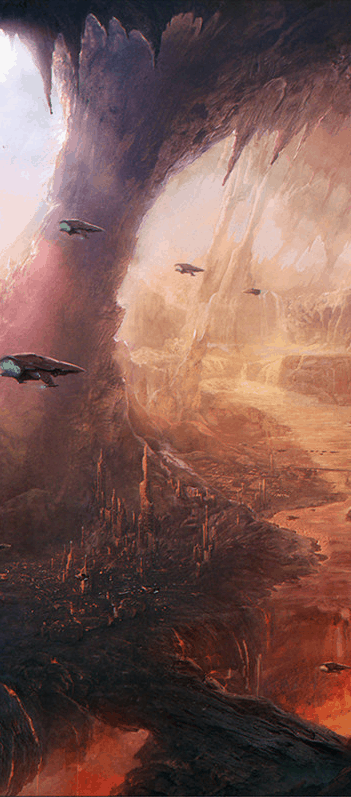
\includegraphics[width=\linewidth]{img/personnages/handicap.png}


\clearpage
\subsection{Atouts}

Voici le liste des Atouts disponibles dans \swfe.

\subsubsection{Background}
\begin{description}[align=left]
    \item [Ambidextre]
    	\emph{[Novice, Agi d8+]}\\
        Votre héros utilise ses deux mains avec la même facilité.

    \item [Arcane (Force)]
    	\emph{[Novice, spécial, \^Ame d8+]}\\
        L'atout indispensable si votre héro doit utiliser la Force.

    \item [Brave]
    	\emph{[Novice, spécial]}\\
        Ceux qui possèdent cet Atout ont appris à maîtriser leurs peurs.

    \item [Chanceux]
    	\emph{[Novice]}\\
        Votre héros semble être béni par le destin.

    \item [Très Chanceux]
    	\emph{[Novice, Chanceux]}\\
        Votre héros semble être béni par le destin. Deux fois.

    \item [Costaud]
    	\emph{[Novice, Force et Vigueur d6+]}\\
        Votre héros est très corpulent ou tout simplement très athlétique.

    \item [Don des langues]
    	\emph{[Novice, Intellect d6+]}\\
        Le personnage a un don pour les langues.

    \item [Enragé]
    	\emph{[Novice]}\\
        Dès qu’il est blessé (ou même Secoué par une attaque physique) votre héros doit réussir un jet d’Intellect sans quoi il devient Enragé. Un personnage enragé attaque sans aucune retenue.

    \item [Guérison rapide]
    	\emph{[Novice, Vigueur d8+]}\\
        Votre héros récupère vite de ses blessures.

    \item [Noble]
    	\emph{[Novice]}\\
        Les personnages de haute naissance sont avantagés par la vie mais ont aussi plus de responsabilités.

    \item [Résistance à la Force]
    	\emph{[Novice, \^Ame d8+]}\\
        Votre héro, même s'il ne sait pas l'utiliser, est capable de résister à la Force quand elle est employé contre lui.

    \item [Grande résistance à la Force]
    	\emph{[Novice, Résistance à la Force]}\\
        Comme précédent mais avec un bonus de résistance double.

    \item [Riche]
    	\emph{[Novice]}\\
        Que votre héros soit né avec une cuillère en argent dans la bouche ou bien qu’il ait bien réussi en affaires, une chose est sûre : il est beaucoup plus fortuné que la plupart des gens.

    \item [Très riche]
    	\emph{[Novice, Riche ou Noble]}\\
        Votre héros est riche comme Crésus.

    \item [Séduisant]
    	\emph{[Novice, Vigueur d6+]}\\
        Votre héros a beaucoup de charme ou est très beau.

    \item [Très séduisant]
    	\emph{[Novice, Séduisant]}\\
        Votre héros est d’une beauté à couper le souffle.

    \item [Véloce]
    	\emph{[Novice, Agilité d6+]}\\
        Le héros se déplace très rapidement.

    \item [Vif]
    	\emph{[Novice, Agilité d8+]}\\
        Votre héros est né avec des réflexes presque surhumains.

    \item [Vigilant]
    	\emph{[Novice]}\\
        Peu de choses échappent à votre héros. Il est vigilant et très observateur.
\end{description}

\begin{paperbox}{Arcane (Force)}
    Remplace l'attout Arcanes. C'est l'atout qui représente la Force, l\^Ame étant assimilé au niveau de maîtrise de la Force.
\end{paperbox}

\begin{paperbox}{Résistance à la Force}
    Comme sont niveau supérieur Grande Résistance à la Force, cet atout remplace la résistance aux Arcanes. il correspond comme son nom l'indique à la capacité que le héro a de résisté à la force.

    Il confère au héro 2 points d’Armure contre les dégâts provoqués par la Force et ainsi qu'un bonus de +2 aux jets pour résister aux effets de ces pouvoirs. Utiliser un pouvoir bénéfique sur le personnage n'implique pas de malus, cet atout ne se déclenche qu'à la volonté du héro.

    Pour la grande résistance, le bonus d'Armure passe à 4.
\end{paperbox}

\subsubsection{Atouts de Combat}
\begin{description}[align=left]
    \item [Arme fétiche]
    	\emph{[Novice, Combat ou Tir d10+]}\\
        Le héros ne jure que par une arme qu’il connaît par c\oe{ur}.

    \item [Arme fétiche adorée]
    	\emph{[Vétéran, Arme fétiche]}\\
        Votre héros n'utilise que cette arme depuis que ces aventures en commencés, il a une histoire avec cette arme et pour rien au monde il ne s'en séparerait.

    \item [Arts martiaux]
    	\emph{[Novice, Combat d6+]}\\
        Ce personnage est entrainé aux techniques de combat à mains nues.

    \item [Maître des arts martiaux]
    	\emph{[Vétéran, Arts martiaux, Combat d10+]}\\
        Le personnage fait des dégâts de For + d6 lors d’une attaque à mains nues.

    \item [Bagarreur]
    	\emph{[Novice, Force d8+]}\\
        Votre héros a l’habitude de cogner avec ses poings, et fort !

    \item [Cogneur]
    	\emph{[Aguerri, Bagarreur]}\\
        Lorsqu’un cogneur obtient une Relance lors d’une attaque à mains nues.

    \item [Balayage]
    	\emph{[Novice, Force d8+, Combat d8+]}\\
        Cet Atout permet au personnage d’attaquer toutes les cibles adjacentes.

    \item [Grand balayage]
    	\emph{[Vétéran, Balayage]}\\
        Même chose que pour Balayage mais sans le malus.

    \item [Blocage]
    	\emph{[Aguerri, Combat d8+]}\\
        Les héros endurcis au corps à corps sont plus habiles à se défendre que les autres.

    \item [Grand blocage]
    	\emph{[Vétéran, Blocage]}\\
        Même chose que pour Blocage mais le bonus est double.

    \item [Combat à deux armes]
    	\emph{[Novice, Agilité d8+]}\\
        Votre héros n’est pas ambidextre mais sait se battre avec deux armes en même temps.

    \item [Combatif]
    	\emph{[Aguerri]}\\
        Votre héros se ressaisit vite après un coup ou une émotion forte.

    \item [Contre-attaque]
    	\emph{[Aguerri, Combat d8+]}\\
        Les combattants disposant de cet Atout sont capables de répondre instantanément aux erreurs de leurs adversaires.

    \item [Grande contre-attaque]
    	\emph{[Vétéran, Contre-attaque]}\\
        Comme contre-attaque, mais sans le malus.

    \item [Dégaine comme l’éclair]
    	\emph{[Novice, Agilité d8+]}\\
        Cet Atout permet au héros de dégainer une arme et d’attaquer dans le même round sans subir de malus.

    \item [Esquive]
    	\emph{[Aguerri, Agilité d8+]}\\
        L’expérience a appris à votre héros comment esquiver les mauvais coups.

    \item [Grande esquive]
    	\emph{[Vétéran, Esquive]}\\
        Même chose que pour Esquive en doublant les effets.

    \item [Extraction]
    	\emph{[Novice, Agilité d8+]}\\
        Votre héros utilise ses deux mains avec la même facilité.

    \item [Grande extraction]
    	\emph{[Novice, Extraction]}\\
        Comme Extraction, mais en cas de Relance sur le jet d’Agilité, aucun adversaire au contact du personnage ne bénéficiera d’une attaque gratuite.

    \item [Florentine]
    	\emph{[Novice, Agilité d8+, Combat d8+]}\\
        Combattre à la Florentine est une technique basée sur l’utilisation de deux armes à la fois.

    \item [Frappe éclair]
    	\emph{[Novice, Agilité d8+]}\\
        Une fois par round votre héros obtient une attaque de Combat gratuite contre un seul ennemi venant au contact.

    \item [Frappe foudroyante]
    	\emph{[Héroïque, Frappe éclair]}\\
        Même chose que pour Frappe éclair, mais le héros obtient une attaque de Combat supplémentaire contre chacun des ennemis venant au contact.

    \item [Frénésie]
    	\emph{[Aguerri, Combat d10+]}\\
        Frénésie en combat de mêlée permet de faire pleuvoir des coups rapides sur ses adversaires au détriment de la précision.

    \item [Frénésie suprême]
    	\emph{[Vétéran, Frénésie]}\\
        Même chose que pour Frénésie mais sans le malus.

    \item [Improvisation martiale]
    	\emph{[Aguerri, Intellect d6+]}\\
        Les héros se trouvent parfois avec du matériel non destiné au combat. Votre héros est capable d’utiliser ce genre d’objets en tant qu’armes improvisées.

    \item [Increvable]
    	\emph{[Joker, Novice, Âme d8+]}\\
        Votre héros a plus de vies qu’un camion rempli de chats.

    \item [Trompe-la-mort]
    	\emph{[Joker, Novice, Âme d8+]}\\
        Votre héros est plus dur à tuer que Raspoutine lui-même.

    \item [Instinct de tueur]
    	\emph{[Héroïque]}\\
        Votre héros déteste perdre. Dans un cas d’égalité sur un jet opposé, il gagne.

    \item [Nerfs d’acier]
    	\emph{[Joker, Novice, Vigueur d8+]}\\
        Même chose que pour Nerfs d’acier, mais 2 points de malus pour blessures sont ignorés.

    \item [Panache]
    	\emph{[Novice, \^Ame d8+]}\\
        Quand ce héros met tout son cœur dans une tache, ça se voit !

    \item [Poigne ferme]
    	\emph{[Novice, Agilité d8+]}\\
        Votre héros ignore le malus Plateforme instable pour tirer depuis un véhicule ou sur une monture en mouvement.

    \item [Rock n’ roll !]
    	\emph{[Aguerri, Tir d8+]}\\
        Les tireurs expérimentés ont appris à maîtriser le recul provoqué par les armes automatiques.

    \item [Sans pitié]
    	\emph{[Aguerri]}\\
        Le personnage peut utiliser un Jeton pour relancer un jet de dégâts, y compris pour une attaque de zone.

    \item [Tête froide]
    	\emph{[Aguerri, Intellect d8+]}\\
        Celui qui garde son calme quand les autres courent aux abris est un adversaire redoutable.

    \item [Sang-froid]
    	\emph{[Aguerri, Tête froide]}\\
        Même chose que pour Tête froide en doublant les effets.

    \item [Tireur d’élite]
    	\emph{[Aguerri]}\\
        Le héros vise juste et bien.

    \item [Tueur de géant]
    	\emph{[Vétéran]}\\
        En général plus c’est grand plus c’est dur à vaincre. Mais votre héros sait trouver les points faibles des créatures de grande taille.

\newpage

    \item [Maître Jedi]
    	\emph{[Vétéran, \^Ame d12+, Padawan]}\\
        Après sa formation et après avoir prété serment à l'ordre, votre héro pourra devenir un Maître Jedi.

    \item [Seigneur Sith]
    	\emph{[Vétéran, \^Ame d12+, Apprenti Sith]}\\
        Votre héro, après avoir prété serment à son Maître, devient à son tour un seigneur Sith.

    \item [Padawan]
    	\emph{[Aguerri, \^Ame d10+, Arcane (Force)]}\\
        La sensibilité de votre héro à la force a été remarqué et l'ordre vous accepte comme padawan sous la tutelle d'un Maître.

    \item [Apprenti Sith]
    	\emph{[Aguerri, \^Ame d10+, Arcane (Force)]}\\
        La haine et la rancoeur de votre héro à donné des idées à un Seigneur Sith qui decide de vous prendre comme apprenti.


\end{description}

\subsubsection{Atouts de commandement}

\begin{description}[align=left]
    \item [Ambidextre]
    	\emph{[Novice, Agilité d8+]}\\
        Votre héros utilise ses deux mains avec la même facilité.

    \item [Ambidextre]
    	\emph{[Novice, Agilité d8+]}\\
        Votre héros utilise ses deux mains avec la même facilité.

    \item [Ambidextre]
    	\emph{[Novice, Agilité d8+]}\\
        Votre héros utilise ses deux mains avec la même facilité.

    \item [Ambidextre]
    	\emph{[Novice, Agilité d8+]}\\
        Votre héros utilise ses deux mains avec la même facilité.

    \item [Ambidextre]
    	\emph{[Novice, Agilité d8+]}\\
        Votre héros utilise ses deux mains avec la même facilité.

    \item [Ambidextre]
    	\emph{[Novice, Agilité d8+]}\\
        Votre héros utilise ses deux mains avec la même facilité.

    \item [Ambidextre]
    	\emph{[Novice, Agilité d8+]}\\
        Votre héros utilise ses deux mains avec la même facilité.

    \item [Ambidextre]
    	\emph{[Novice, Agilité d8+]}\\
        Votre héros utilise ses deux mains avec la même facilité.

    \item [Ambidextre]
    	\emph{[Novice, Agilité d8+]}\\
        Votre héros utilise ses deux mains avec la même facilité.


\end{description}

\newpage
\subsection{Création du personnage}

\subsubsection{Race}
Choisissez la race de votre personnage parmi celles proposées.

\subsubsection{Traits}
\begin{itemize}
	\item Votre héros débute avec un d4 dans chaque Attribut et dispose de 5 points avec lesquels il peut les augmenter. Augmenter un Attribut d’un type de 	dé coûte 1 point.
	\item Vous avez 15 points pour vos Compétences.
	\item Chaque type de dé investi dans une Compétence coûte 1 point jusqu’à égaler le dé de l’Attribut dont dépend la Compétence. Au-delà, le coût est de 	2 points.
	\item Le Charisme est égal au total des bonus ou des malus donnés par les Atouts ou les Handicaps.
	\item L’Allure est de 6 cases.
	\item La Parade est égale à 2 plus la moitié de la Compétence Combat.
	\item La Résistance est égale à 2 plus la moitié de Vigueur. Vous pouvez y ajouter le bonus de l’armure portée sur le torse pour accélérer le calcul en 	cours de partie mais ce bonus ne compte pas pour les autres parties du corps.
\end{itemize}

\subsubsection{Atouts \& Handicaps}
Vous gagnez des points supplémentaires en prenant un Handicap Majeur (2 points) et jusqu’à deux Handicaps Mineurs (1 point chacun).

Pour 2 points vous pouvez :
\begin{itemize}
	\item Augmenter un Attribut d’un type de dé.
	\item Choisir un Atout.
\end{itemize}

Pour 1 point vous pouvez :
\begin{itemize}
	\item Augmenter une Compétence d’un type de dé.
	\item Doubler vos fonds initiaux.
\end{itemize}

\subsubsection{Équipement}
Débutez avec 500 Cr.

\subsubsection{Histoire personnelle}
Rajoutez les détails concernant le personnage qui vous semblent importants.

\subsection{Progression}
Le rang détermine la puissance approximative de votre héros. Le nombre de points d’XP que vous avez gagné détermine le rang selon le tableau suivant : \\

\begin{tabular}{ l l }
	\textbf{XP}		& \textbf{Rang} \\
	\hline
	00-19 			& Novice \\
   	20-39 			& Aguerri \\
   	40-59 			& Vétéran \\
   	60-79 			& Héroïque \\
   	80+				& Légendaire
\end{tabular}
\\

Tout les 5XP votre héros bénéficie d’une progression. Lors d’une progression il peut :
\begin{itemize}
	\item Choisir un nouvel Atout.
	\item Augmenter une Compétence dont la valeur est égale ou supérieure au Trait associé.
	\item Augmenter deux Compétences dont les valeurs sont inférieures aux Traits associés.
	\item Prendre une nouvelle Compétence à d4.
	\item Augmenter un Attribut d’un type de dé. Vous ne pouvez choisir cette option qu’une fois par Rang ou lors d’une progression sur deux après avoir atteint le rang Légendaire. Il n’est pas possible de progresser au-delà de d12 dans un Trait par le biais d’une Progression, mais vous pouvez consulter les Atouts Professionnel~\ref{sec:atout-professionnel} et Expert~\ref{sec:atout-expert} (p.~\pageref{sec:atout-professionnel}).
\begin{itemize}

\clearpage 

